\documentclass{standalone}
\usepackage{../preamble}

\begin{document}
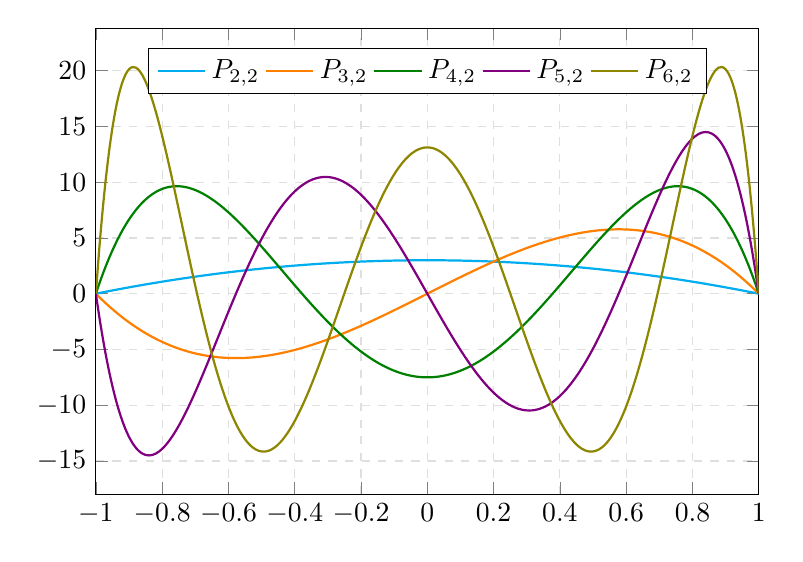
\begin{tikzpicture}
  \begin{axis}
    [
      xmin = -1, xmax = 1, %
      % ymin = -1.1, ymax = 1.2, %
      % xtick distance = 0.5, %Is the distance between major ticks in the x-axis.
      ytick distance = 5, %Is the distance between major ticks in the y-axis.
      % minor tick num = 1, %Is the number of ticks between major ticks.
      grid=major,
      major grid style = {lightgray!50, dashed}, %Changes the color and stroke of the major grid.
      minor grid style = {lightgray!25}, %Changes the color and stroke of the minor grid.
      width = 10cm, %sets the width of the figure
      height = 7.5cm,  %sets the height of the figure
      xlabel = {}, %
      ylabel = {}, %
      legend cell align = {left}, %
      legend columns=5,
      legend style={at={(axis cs:0,20)},anchor=center} % position of the legend box and anchor is the point on the box to be fitted exactly at the point of cs:<>,<>. Options are anchor=center,south west,south east,north west,north east,north,south,west...
    ]
    \addplot[
      domain=-1:1, %Domain of the fucntion
      samples=200, %This parameter determines the number of point to be plotted for the function, while bigger the number better looks the function.
      smooth, %f we use this option, the compiler makes an interpolation between the point plotted to get a soft appearance for the function.
      thick, %Stroke of the function. Options: ultra thin, very thin, thin, semithick, thick, very thick, ultra thick.
      cyan %Color of the function.
    ]{3*(1-x^2)};
    \addplot[
      domain=-1:1, %Domain of the fucntion
      samples=200, %This parameter determines the number of point to be plotted for the function, while bigger the number better looks the function.
      smooth, %f we use this option, the compiler makes an interpolation between the point plotted to get a soft appearance for the function.
      thick, %Stroke of the function. Options: ultra thin, very thin, thin, semithick, thick, very thick, ultra thick.
      orange %Color of the function
    ]{15*x*(1-x^2)};
    \addplot[
      domain=-1:1, %Domain of the fucntion
      samples=200, %This parameter determines the number of point to be plotted for the function, while bigger the number better looks the function.
      smooth, %f we use this option, the compiler makes an interpolation between the point plotted to get a soft appearance for the function.
      thick, %Stroke of the function. Options: ultra thin, very thin, thin, semithick, thick, very thick, ultra thick.
      green!50!black %Color of the function
    ]{15/2*(7*x^2-1)*(1-x^2)};
    \addplot[
      domain=-1:1, %Domain of the fucntion
      samples=200, %This parameter determines the number of point to be plotted for the function, while bigger the number better looks the function.
      smooth, %f we use this option, the compiler makes an interpolation between the point plotted to get a soft appearance for the function.
      thick, %Stroke of the function. Options: ultra thin, very thin, thin, semithick, thick, very thick, ultra thick.
      violet %Color of the function
    ]{105/2*x*(3*x^2-1)*(1-x^2)};
    \addplot[
      domain=-1:1, %Domain of the fucntion
      samples=200, %This parameter determines the number of point to be plotted for the function, while bigger the number better looks the function.
      smooth, %f we use this option, the compiler makes an interpolation between the point plotted to get a soft appearance for the function.
      thick, %Stroke of the function. Options: ultra thin, very thin, thin, semithick, thick, very thick, ultra thick.
      olive %Color of the function
    ]{105/8*(33*x^4-18*x^2+1)*(1-x^2)};
    \legend{$P_{2,2}$,$P_{3,2}$,$P_{4,2}$,$P_{5,2}$,$P_{6,2}$}
  \end{axis}
\end{tikzpicture}
\end{document}